\documentclass{article}
\usepackage[utf8]{inputenc}
\usepackage{amsmath, amssymb, amsthm}
\usepackage{graphicx, float}
\graphicspath{ {./imagens/} } 
\usepackage{multicol}
\usepackage[brazil]{babel}
\usepackage{pgfplots}
\pgfplotsset{compat=1.18}
\usepackage[letterpaper, top = 1in, bottom = 1.0 in, left = 1.2 in, right = 1.2 in, heightrounded]{geometry}

%%%%%%%%%%%%%%%%%%%%%%%%% Caso haja dúvidas na Symbologia %%%%%%%%%%%%%%%%
% https://detexify.kirelabs.org/classify.html
% https://app.mettzer.com/latex
%%%%%%%%%%%%%%%%%%%%%%%%% Parâmetros de construção %%%%%%%%%%%%%%%%%%%%%%%
\setlength{\parindent}{0pt}
\setlength{\parskip}{0.8em}

\title{\textbf{Repositório de Estatistica e Probabilidade}}
\author{UFSC Joinville - EMB5010 \\ Artur Gemaque}
\date{\today}
%%%%%%%%%%%%%%%%%%%%%%%%%% COMEÇO DO DOCUMENTO %%%%%%%%%%%%%%%%%%%%%%%%%%%
\begin{document}
\maketitle

\begin{abstract}
Este documento tempo como principal funcionalidade registrar os contudos ensinados 
em sala de aula pelo professor Jaimes, ademais servirá como fonte de estudo para as 
provas referentes há Matéria.
\end{abstract}

\section{Análise Exploratória de Dados}

    \begin{multicols}{2}
    
        Vamos começar com as definições mais simplórias da matéria que são resultado do cálculo dos dados.

        \subsection{Média}
        \ A média aritmética de um conjunto de n números é a soma desses números dividida por n.
          \begin{center}
            $ \overset{\_}{x} =  \overset{n}{\underset{i=1}{\sum}} \frac{X_i}{n}  $
          \end{center}

        \subsection{Variância}
        \ A variância é um conceito fundamental em estatística que mede a dispersão de um conjunto de dados em relação à sua média.
          \begin{center}
            $ (S)^2 =  \frac{\overset{n}{\underset{i=1}{\sum}} (X_i - \overset{\_}{x} )^2 }{n - 1} $
          \end{center}

        \subsection{Desvio padrão}
        \ O desvio padrão é uma medida de dispersão estatística que indica o quão afastados os 
        dados de um conjunto estão da sua média. Ele é a raiz quadrada da variância, o que o 
        torna mais interpretável.
          \begin{center}
            $ S = \sqrt[2]{S^2}$
          \end{center}

        \subsection{Valores de análise}
        \ Partindo agora para valores que são obtidos apartir dos dados ordenados em formato crescente. 
        Observação que as seguintes fórmulas serão para que possamos obter as posição dos referidos valores.    
        \subsection{Mediana}
        Mediana é o número no centro de um grupo de números.
        \begin{center}
          $ Md = X_{\left(\frac{n + 1}{2}\right)} $
        \end{center}

        \subsection{Quartis}
        \ Os quartis são valores que dividem uma amostra de dados em quatro partes iguais e são usados para 
        avaliar a dispersão e a tendência central de um conjunto de dados. Eles são os valores contidos nas 
        posições de $ n*25\% $ entre outras porcentagens, caso "n" dê um valor quebrado o Quartil vai ser a 
        média entre os dois valores.
        \begin{center}
          $ Q_1 = X_{\left(\frac{n + 1}{4}\right)} $ \\
          $ Q_3 = X_{\left(\frac{3(n + 1)}{4}\right)} $
        \end{center}

        \subsection{Moda}
        \ A moda é o valor que mais aparece em um conjunto de dados, ou seja, o valor que tem maior frequência.

        \subsection{Amplitude}
        \ A amplitude de um conjunto de dados é a diferença entre o maior e o menor valor. Para calcular a amplitude, 
        subtrai-se o menor valor do maior. 

        \subsection{Histograma}
        \ Um histograma é uma espécie de gráfico de barras que demonstra uma distribuição de frequências. No histograma, 
        a base de cada uma das barras representa uma classe e a altura representa a quantidade ou frequência absoluta com 
        que o valor de cada classe ocorre.

        \hbox{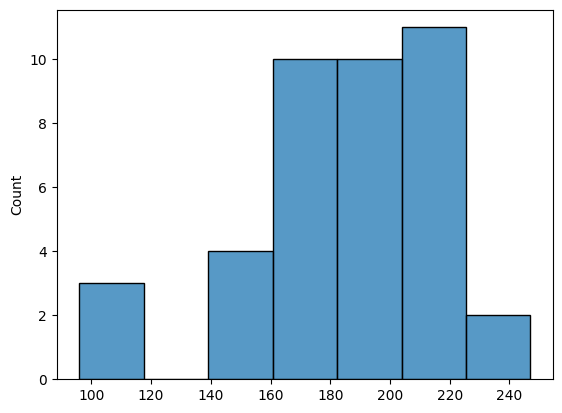
\includegraphics[width=7cm]{Histograma.png}}

        \subsection{Boxplot}  
        \ O Box Plot, que estudamos no curso Green Belt, é uma ferramenta gráfica que ajuda a identificar a existência de 
        possíveis outliers no conjunto de dados. Em um boxplot são apresentadas 5 estatísticas: o mínimo, o primeiro quartil 
        (Q1), a mediana, o terceiro quartil (Q3) e o máximo.

        \hbox{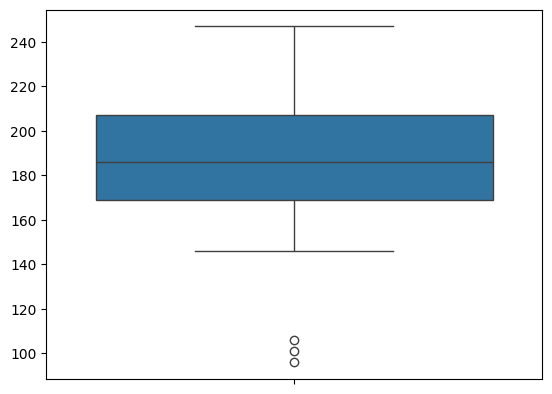
\includegraphics[width=7cm]{Boxplot.png}}  

    \end{multicols}

    \newpage
    
\section{Probabilidade}
    
    \subsection{Conceitos Introdutórios}

        \ O conceito de "Modelo Probabilístico" consiste contém variáveis aleatórias, 
        dadas as entradas não se há certeza das saídas. Em contra partida ao modelo deterministíco 
        que contém dado os valores de entrada se tem certeza dos valores de saída. Exemplo:
        \begin{itemize}
            \item $ F = m*a $
            \item $ v = \frac{\Delta x}{\Delta t} $
            \item $ M_f = M_i (1 + i)^n $ 
        \end{itemize}
    
    
        \ O "Experimento Aleatório" pode ser entendido como o experimento que pode fornecer diferentes resultados,
        embora seja repetido da mesma maneira, este por sua vez é feito dentro de um conjuntos de possibilidades
        que podemos chamar de "Espaço Amostral", ou conjunto de todos os possíveis resultados de um experimento
        aleatório, podendo ser classificado em "Espaço amostral discreto" quando conjunto finito ou "Espaço amostral 
        contínuo" quando os possíveis resultados representam um intervalo de números reais. Por fim,
        entendemos por "Evento" um subconjunto do espaço amostral, um resultado ou combinação de
        resultados do experimento aleatório.


        \ Probabilidade condicional é quando um evento tem uma condição fixa para que aconteça, ou seja, para um dado
        espaço amostral $ \Omega $ em que dois dados sejam lançados aleatoriamente uma probabilidade condicional seria
        que todos os eventos que buscamos sejam quando a soma do D1 com D2 seja sempre 8, isto representaria uma 5 de 36 possibilidades.

        \begin{itemize}
            \item $ P( D1+D2 = 8 ) = \frac{N-de-Eventos}{Espaco-Amostral} = \frac{5}{36} $
        \end{itemize}
    \subsection{Axiomas da Probabilidade}

        \begin{multicols}{2}

        \ Sejam $ A_i $ num espaço amostral $ \Omega: $
        \begin{itemize}
          \item $ 0 \leqslant P(A_i) \leqslant 1 $
          \item $ P(\Omega) = 1 $
          \item $ P(A_1 \bigcup A_2) = P(A_1) + P(A_2)\\ \because P(A_1 \cap A_2) = 0 $
        \end{itemize}
        
        \ Algumas propriedades decorrentes dos axiomas:
        
        \begin{itemize}
          \item $ P( \varnothing ) = 0 $
          \item $ P(A) + P(\overset{\_}{A}) = 1 \ \rightarrow P(\overset{\_}{A}) = 1 - P(A) $
          \item $ P(A_1 \bigcup A_2) = P(A_1) + P(A_2) - P(A_1 \cap A_2) $
        \end{itemize}

        \end{multicols}

    \begin{center}
        \ Função probabilidade $ P(x) $ e Função probabilidade Acumulada $ F(x) $
        {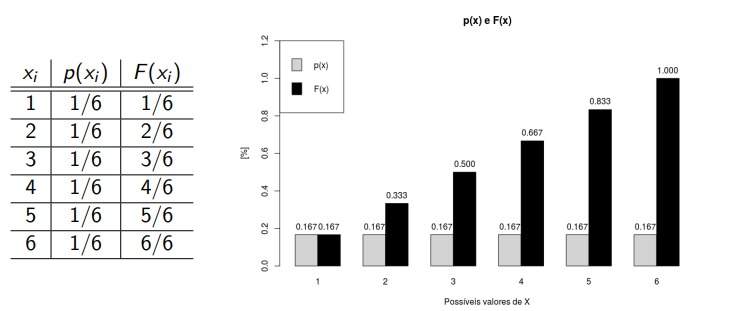
\includegraphics[width=12cm]{Função Prob e Prob Acumulada.jpg}}
    \end{center}
      
    \newpage

\section{Variáveis Aleatórias Discretas}

  \ Dentro dos conceitos definidos anteriormente de VAD (Variáveis Aleatórias Discretas), exitem as principais distribuições discretas como Bernoulli, que 
  compreende a probabilidade de sucesso como $ P $ e o fracasso como $ 1-P $ além das distribuições Binomial e de Poisson.
  
  \subsection{Distribuição Binomial}

  \begin{multicols}{2}

  Existem algumas condições para aplicação de tal distribuição
  \begin{itemize}
    \item Os ensaios sejam independentes
    \item Caso haja somente dois resultados possíveis: Sucesso ou fracasso
    \item A probabilidade de sucesso (p) seja constante
    \item X = Número de ensaios que resultam em sucesso
    \item n = Número de ensaios realizados
  \end{itemize}

  Definição como distribuição Binomial:

  \begin{Large}
  \begin{quote}
    \hbox{
    $ p(x) = \left( \frac{n!}{(n-x)!x!} \cdot p^x \cdot (1-p)^{n-x} \right)$}
  \end{quote}
  \end{Large}
  
  Calculo de $ \mu $ e $ \sigma^2 $:
 
  \begin{itemize}
    \item $ \mu = n \cdot p $
    \item $ \sigma = \sqrt{n \cdot p \cdot (1 - p)} $
  \end{itemize}  
  \end{multicols}

  \subsection{Distribuição de Poisson}

  \ A variável aleatória X, que é igual ao número de ocorreências no intervalo

  \begin{LARGE}
    \begin{quote}
      $ p(x) = \frac{  e^{- \lambda T} \cdot (\lambda T)^x }{x!} $
    \end{quote}
    \end{LARGE}

  \begin{itemize}
    \item $x$ = número de ocorreências no intervalor de tamanho $ T $
    \item $\lambda$ = taxa de ocorreências (constante)
    \item $e$ = número de Euler (constante)
  \end{itemize}

  \ Média e variância

  \begin{itemize}
    \item $\mu = \lambda T $
    \item $\sigma^2 = \lambda T$
  \end{itemize}
  
\newpage

\section{Variáveis Aleatórias Contínuas}

  \subsection{Função de Densidade de Probabilidade}

  \begin{multicols}{2}
  
    \hbox{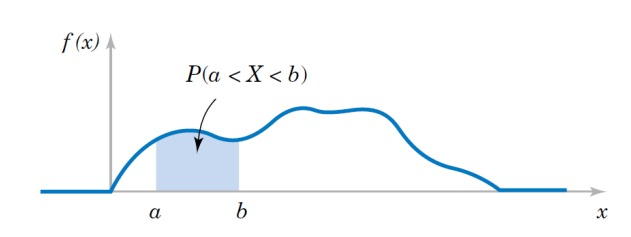
\includegraphics[width=8cm]{Função Densidade.jpg}}
    \begin{itemize}
      \item $ f(x) \geqslant 0 $ 
      \item $ \int^{\infty}_{-\infty} f(x)dx = 1$
      \item $ P(a \geqslant X \geqslant b) = \int^{b}_{a} f(x)dx $
    \end{itemize}

  \end{multicols}
  
  \ Comparação entre a Média e a Variância

  \begin{multicols}{2}
    
    Média e Variância de uma VAD
    \begin{itemize}
      \item $ E(x) = \overset{n}{\underset{i=1}{\sum}} x_i \cdot p_i $
      \item $ V(x) = \overset{n}{\underset{i=1}{\sum}} (x_i - \mu )^2 \cdot p_i $
    \end{itemize}
    
    Média e Variância de uma VAC
    \begin{itemize}
      \item $ E(x) =  \int^{\infty}_{-\infty} x \cdot f(x)dx$
      \item $ V(x) =  \int^{\infty}_{-\infty} (x-\mu)^2 \cdot f(x)dx$
    \end{itemize}
  
  \end{multicols}

  \subsection{Distribuição Uniforme}

  \begin{multicols}{2}

    \hbox{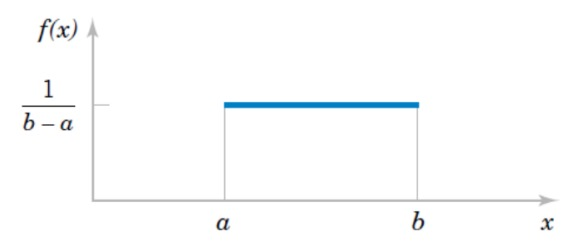
\includegraphics[width=8cm]{distribuição continua.jpg}}  
    \begin{itemize}
      \item $ f(x) = \frac{1}{b-a}$
      \item $ \mu = \frac{a+b}{2} $
      \item $ \sigma^2 = \frac{(b-a)^2}{12}$
    \end{itemize}

  \end{multicols}
  
  \subsection{Distribuição Exponecial}

  \begin{multicols}{2}

    \hbox{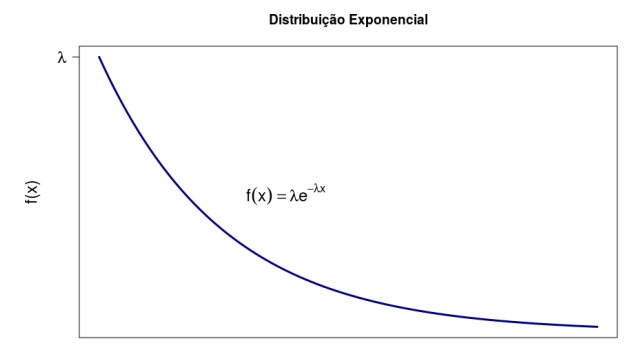
\includegraphics[width=8cm]{Distribuição exponelcial.jpg}}

    \begin{itemize}
      \item $ f(x) = \lambda e^{-\lambda T}$
      \item $ \mu = \frac{1}{\lambda} $
      \item $ \sigma^2 = \frac{1}{\lambda^2}$
    \end{itemize}

  \end{multicols}

  \subsection{Distribuição Normal}
  \begin{center}
    $ Z = \frac{X - \mu}{\sigma} \rightarrow $ O resto é tabela Tmj S2
  \end{center}

\end{document}